\documentclass[12pt]{article}
\usepackage[utf8]{inputenc}

\usepackage{amsfonts}
\usepackage{amssymb}
\usepackage{amsmath}
\usepackage{amsthm}
\usepackage{enumitem}

\usepackage{graphicx}

\usepackage{bbold}
\usepackage{bm}
\usepackage{color}
\usepackage{hyperref}
\usepackage[margin=2.5cm]{geometry}

\usepackage{fancyhdr}

\usepackage[english]{babel}
\usepackage[T1]{fontenc}

\begin{document}

% ==============================================================================

\title{Socket Programming : Broker Implementation}								% Title
\author{Romain LAMBERMONT, Arthur LOUIS}								% Author
\date{\today}											% Date

\makeatletter
\let\thetitle\@title
\let\theauthor\@author
\let\thedate\@date
\makeatother

\pagestyle{fancy}
\fancyhf{}
\rhead{\theauthor}
\lhead{\thetitle}
\cfoot{\thepage}

\begin{titlepage}
\centering
	\vspace*{0.5 cm}
	
\includegraphics[scale = 0.7]{facsa.png}\\[1.0 cm]	% University Logo
	\textsc{\LARGE \newline\newline Faculté des Sciences appliquées}\\[2.0 cm]	% University Name
\textsc{\Large  INFO0010-4 : Introduction to Computer Networking}\\[0.5 cm]				% Course Code
\rule{\linewidth}{0.2 mm} \\[0.4 cm]
{ \huge \bfseries \thetitle}\\
\rule{\linewidth}{0.2 mm} \\[1.5 cm]

\begin{minipage}{0.5\textwidth}
	\begin{flushleft} \large
		\emph{Teacher :}\\
		Guy LEDUC\\
		\vspace{0.5cm}
		\emph{Assistant :}\\
		Emeline MARECHAL\\
		\end{flushleft}
		\end{minipage}~
		\begin{minipage}{0.4\textwidth}

		\begin{flushright} \large
		\emph{Group :} \\
		Romain LAMBERMONT\\
		Arthur LOUIS\\
	\end{flushright}

\end{minipage}\\[2 cm]


	\thedate
\end{titlepage}

% ==============================================================================
\thispagestyle{empty}
\tableofcontents
\pagebreak
\setcounter{page}{1}

\section{Introduction}
In this project, we implemented a Broker to handle MQTT messages to communicate with IoTs sensors 
and Subsribers to implement the Monster Hunting Game. In this small report, we'll explain the architecture of our implementation, 
what class we have used and for what purpose. We'll then reflect on MQTT quality of service. We'll finally check what are the limits of our implementation and what we could have done better, 
to implement new features in our MQTT management.

\section{Software architecture}
When starting our project, we had no idea of how to implement the Broker, so we began to sketch our architecture, 
representing the Broker, IoTs sensors and Subscriber. We then started to add our classes one by one to make everything communicate. 
The sketch made it easier to implement everything we wanted and what we should do in each class to make the Game run on the Subscribers. 
The architecture is as follows, to start we launch a \textbf{Broker}, when a new connection enters, it creates a new \textbf{Client} and we handle it 
with \textbf{Messages} that we can \textbf{Receive} and \textbf{Send}. To remember what a client is interested about, there are \textbf{Topics} a client 
can subscribe to.
\\\\

Here is the final sketch of our implementation : 

\begin{figure}[!h]
	\centering
	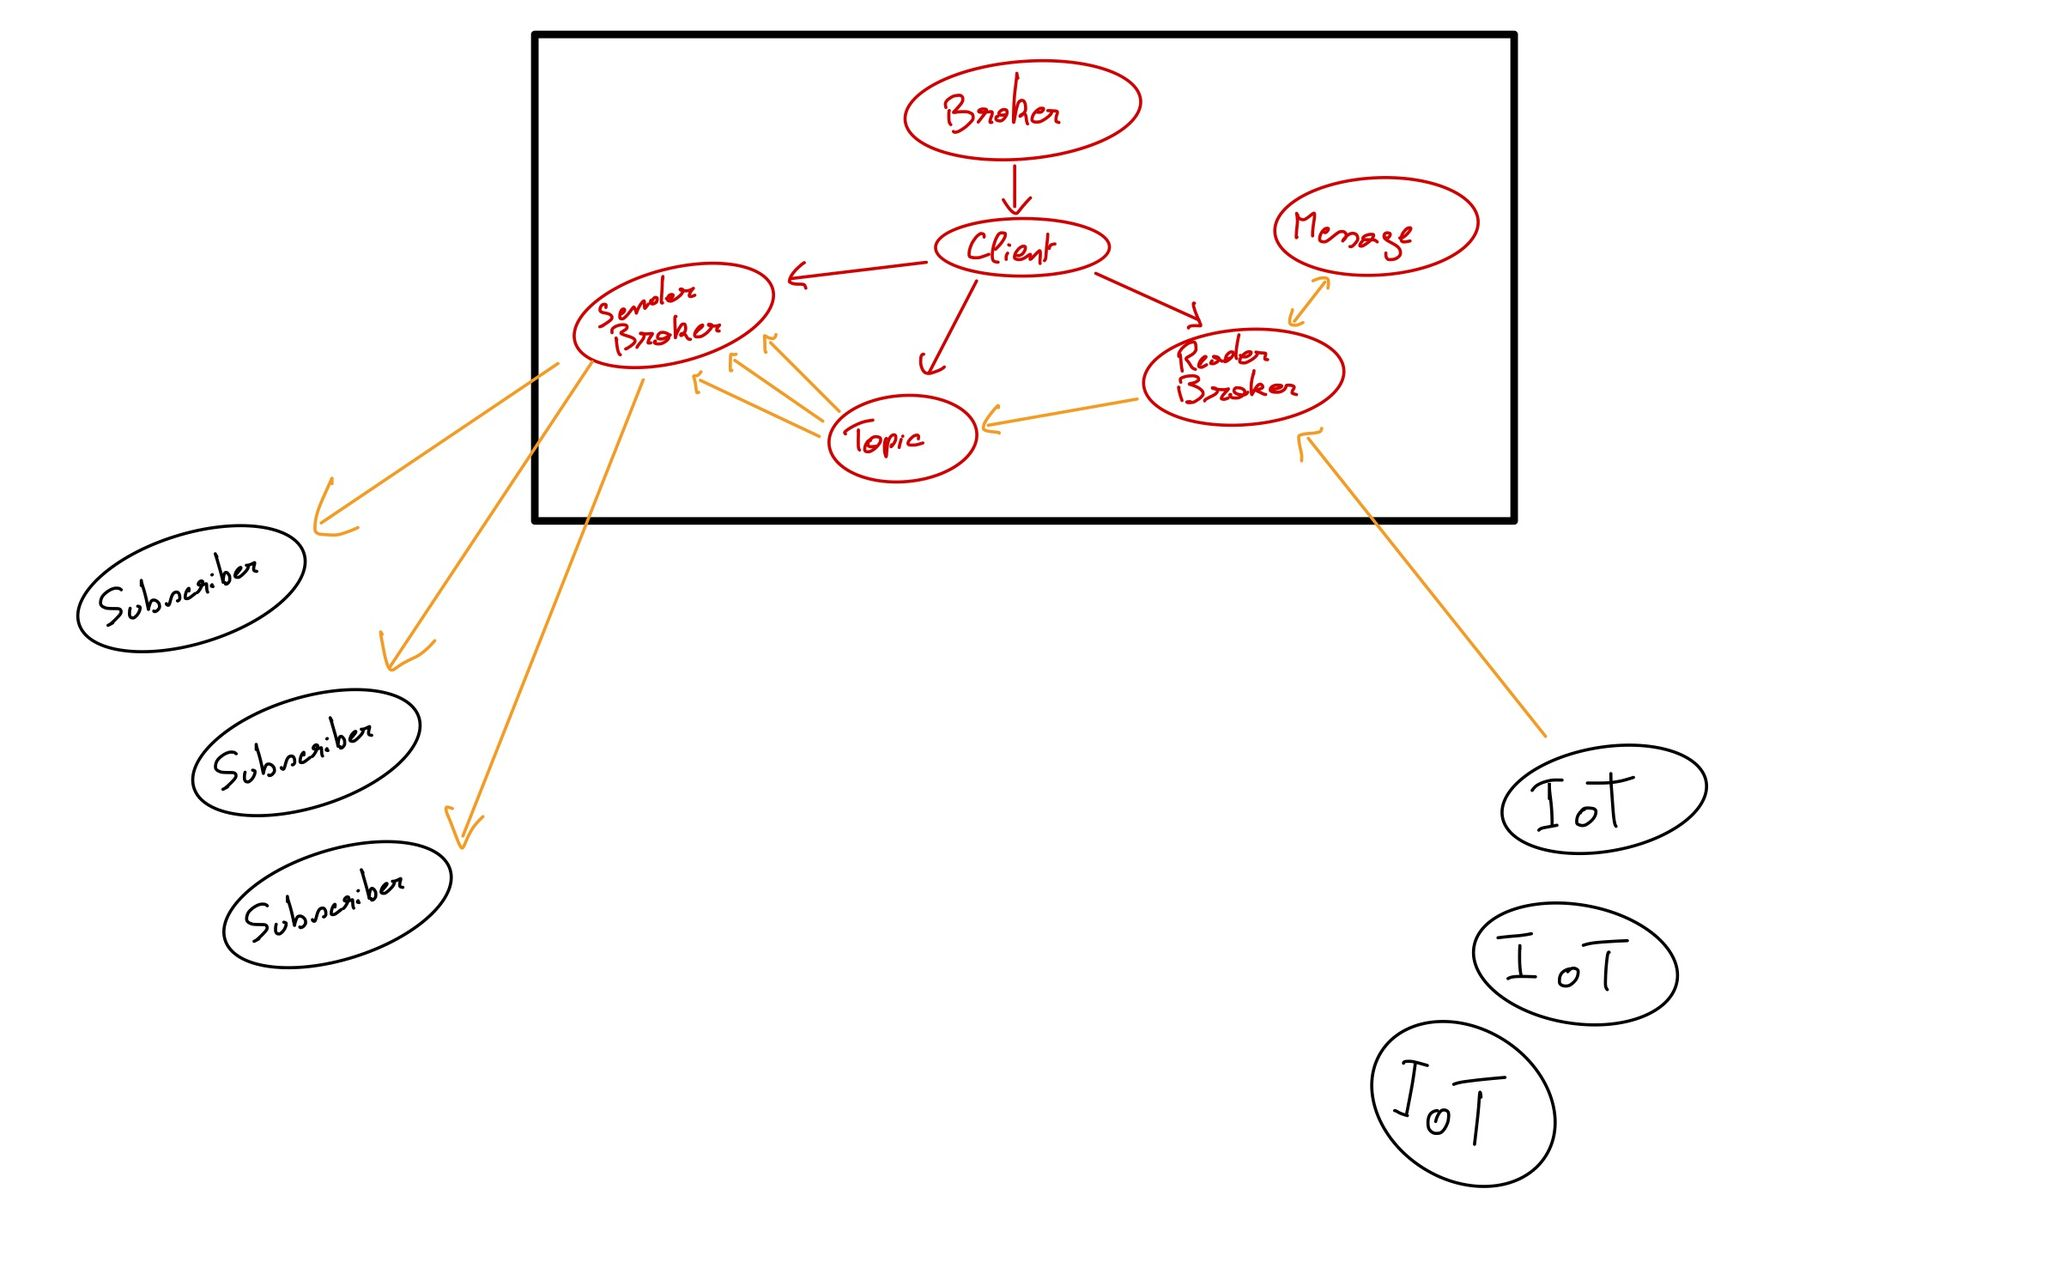
\includegraphics[scale = 0.22]{PublishMessage.jpg}
	\caption{Publish message handeld by our implementation}
\end{figure}

To conclude this first section, here is a reminder of our classes :
\begin{itemize}
	\item \textbf{Broker.java} : Accepts new connections using a ServerSocket and instantiates each needed class. After accepting a connection, it delegates 
	the corresponding Client to the \textbf{Client} class.
	\item \textbf{Client.java} : Receives a Socket and divides in two to \textbf{Send} and \textbf{Receive}.
	\item \textbf{ReaderBroker.java} : Receives packets and handle them to create the corresponding messages to \textbf{Send}.
	\item \textbf{SenderBroker.java} : Sends the response of received packets handeld by \textbf{ReaderBroker.java}.
	\item \textbf{Topic.java} : Stores the \textbf{Clients} interested in specified topics.
	\item \textbf{Message.java} : MQTT toolbox used to decode \textbf{received} packets and to compose new ones to \textbf{send}.
\end{itemize}

\section{Reflection on MQTT's quality of service}
MQTT uses TCP/IP as the protocol to exchange packets and in TCP, there's no loss or alteration of the transmitted data. However, if the TCP connection 
closes (e.g crash or client restart) a totally new TCP connection needs to be created. Without QoS 1 (at least once delivery), in case of a crash of a connection, 
the conversation between server and client would need to restart from as in the case of QoS 1, the conversation can keep on as if nothing append.

\section{Limits \& Possible Improvements}
In this implementation, we created the simplest MQTT Broker possible. Indeed, there's no advanced features that are available in MQTT protocol, namely, Persistant Session, 
Retained Messages and the Last Will and Testament (our Broker is only QoS 0). However, this Broker is only used locally (localhost), so the risk of loss or deformation in packets is almost zero. 
The more advanced features mentionned above would be necessary if our Broker was used online or with a different IoTs/Subscribers structure. 
% ==============================================================================

\end{document}